\section{Introduction}\label{sec:intro}

The Hubbard model appeared in 1963 as one of the first attempts to include electron correlation effects in a quantum mechanical description of a solid \cite{Hubbard1963}. Originally, it was introduced to explain the behavior of the electrons occupying the narrow, partially filled $d-$bands of transition metals. Correlation phenomena in these bands lead to a behavior reminiscent of the atomic picture of a solid. In fact, the Hubbard model may simply be regarded as a minimal model of interacting electrons in an energy band of a solid. We have come a long way since the introduction of the Hubbard model and it is now as paradigm-defining in many-body theory as the Ising model in statistical physics\cite{Mahan2000}.

\begin{figure}[H]
	\centering
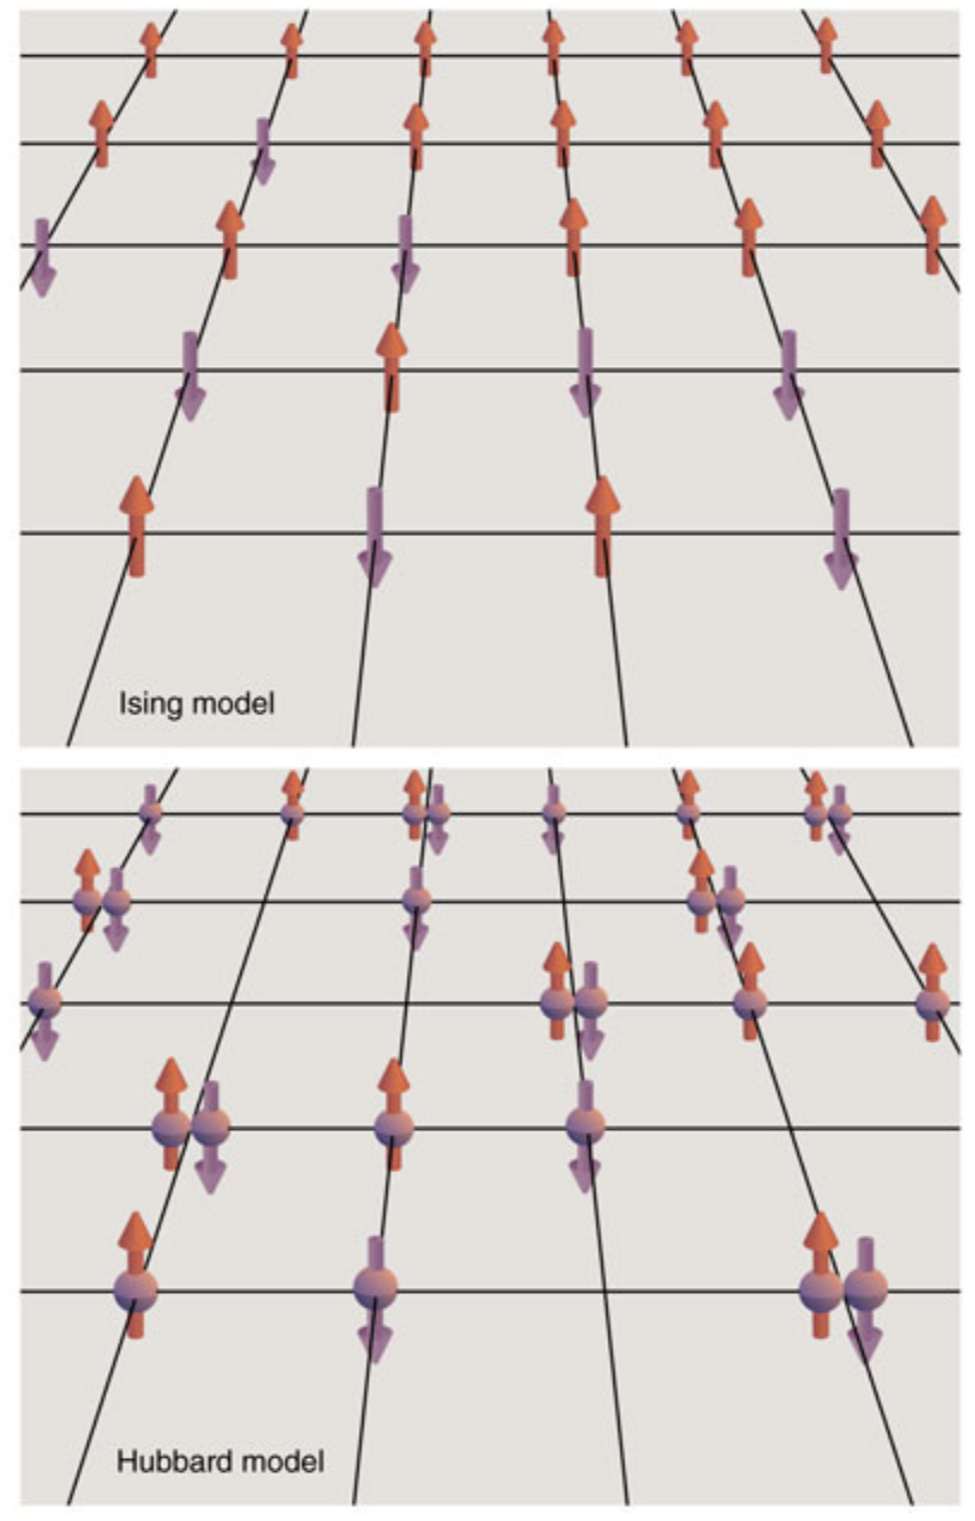
\includegraphics[width=0.5\linewidth]{Figures/3.HubbardModel/isingVsHubbard}
	\caption[Graphical comparison between the Ising and the Hubbard model.]{hi}
	\label{fig:dummyfigure1}
\end{figure}

Unlike the Ising model, where either an up or a down spin live at each site, in the Hubbard model each site can have either no spin, either an up or a down spin, or both.

When Hubbard's seminal paper came out, it followed a trend that arose in the 1950's when people were working on a theory of correlation effects in the free electron gas \cite{Bohm1953, Gell-Mann1957, Sawada1957, Hubbard1957, Hubbard1958, Nozieres1958}. Hubbard devised a simple model for the seemingly intractable problem of interacting electrons in a band. His work explained qualitatively some properties of transition and rare-earth metals in which electron correlations are non negligible. It turns out that the mathematical formulation of the interaction problem for correlated electrons in a band is not prohibitively complicated, and is relatively amenable to both analytical and numerical computations after some reasonable approximations are introduced. Notably, the model is particularly adapted to computer simulations because of its simple approximate Hamiltonian. Moreover, it has been shown to be very relevant in the description of Mott insulators, and high $T_c$ superconductors. In fact, the Hubbard model has found many applications, describing successfully a variety of quantum systems\cite{Editorial2013}; nonetheless, even the simplified picture it offers is in general difficult to approach analytically. There exists an exact solution in one dimension via Bethe ansatz\cite{Lieb1968}, but the more general higher dimensional case is often solved numerically.  Moreover, the solution obtained analytically is not very transparent, and it is hard to extract physical interpretations. An example of particular relevance for the work of this thesis is the study carried out by Hirsch \cite{Hirsch1985}. In the following chapters, we will discuss how to simulate the Hubbard model using a numerical approach that is based on this seminal paper, and in many ways follows the ideas introduced in it.

